\documentclass{beamer}

\usepackage[utf8]{inputenc}
\usepackage{default}


\title[Kurzform]{A State Visualisation Tool} 
\subtitle[Kurzform]{Arranging Quarks} 
\author[Kurzform]{Robert Czechowski, Fabian Wilk} 
\institute[Kurzform]{CERN} 
\date[Kurzform]{04. 08. 2013} 
%\titlegraphic{\includegraphics[width=0.4\textwidth]{../unigoelogo.pdf}}

\begin{document}

\frame{\titlepage}

\frame{
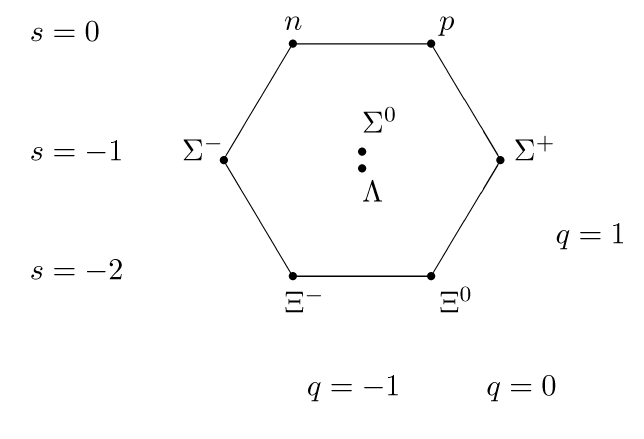
\includegraphics[width=.4\textwidth]{Baryon_octet.png}
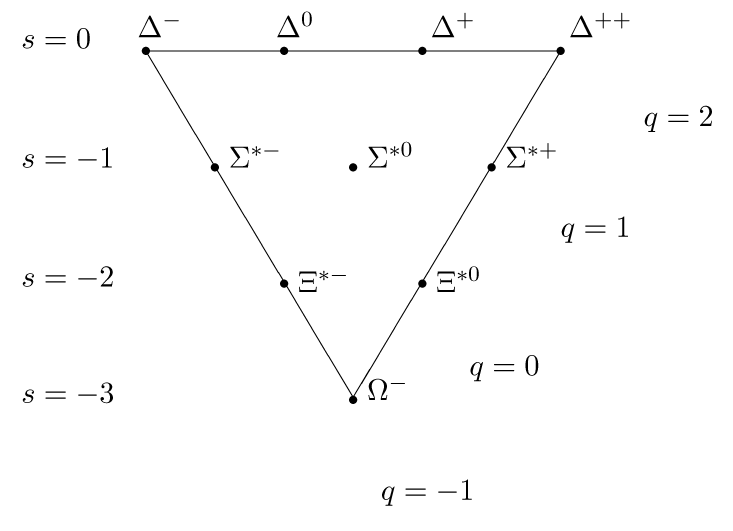
\includegraphics[width=.4\textwidth]{Baryon_decuplet.png}

From [1].

Why are some combinations not possible in the octed?
}

\frame{
Has to do with spin and symmetry of states.

What would be cool: A visualisation of states to see how they look like, and how they transform according to various symmetry operators.
}
\frame{
We did this.
}

\frame{
Written in C++ (CGI) / HTML (+CSS). 
}

\end{document}
